\documentclass{article}
\usepackage{graphicx,wrapfig,hyperref,pdfpages,geometry,amsmath,longtable,eurosym,listings,textcomp}

%substitute "{\em PowerEnJoy}" with "\pej"
\newcommand{\pej}{\mbox{\normalfont\itshape PowerEnJoy }}
%substitute "{\em CSGestion}" with "\csg"
\newcommand{\csg}{\mbox{\normalfont\itshape CSGestion }}
\newcommand{\version}{\mbox{\normalfont v. 1.0 }}

%to keep the links of the TOC invisible
\hypersetup{
	colorlinks,
	citecolor=black,
	filecolor=black,
	linkcolor=black,
	urlcolor=black
}

\geometry{margin=1in}



\begin{document}

	%---------------------------	FRONT PAGE      	-----------------------------
	\title{Politecnico di Milano\\A.A. 2016/2017\\Software Engineering 2: ``{\em PowerEnJoy}'' \version \\ \bigskip \textbf{P}roject \textbf{P}lan }
	\author{Matteo Bresich (mat. 774366)}
	
	
	%to avoid the hyphenation of the name
	\hyphenation{PowerEnJoy}
	
	\begin{figure}[t]
		\centering
		\includegraphics[width=\linewidth]{"img/logo-polimi"}
		\label{fig:polimi-logo}
	\end{figure}

	\maketitle
	
	%BLANK-PAGE
	\thispagestyle{empty}
	\clearpage\mbox{}\thispagestyle{empty}\clearpage
	
	\renewcommand*\thesection{\arabic{section}}
	\renewcommand*\thesubsection{\arabic{section}.\arabic{subsection}}
	\renewcommand*\thesubsubsection{%
		\arabic{section}.\arabic{subsection}.\arabic{subsubsection}%
	}
	\setcounter{secnumdepth}{4}
	\setcounter{tocdepth}{4}
	
	%---------------------------	TABLE OF CONTENT	-----------------------------
	%to change the page numbering from roman in the toc to arabic
	\pagenumbering{roman}
	\renewcommand{\contentsname}{Table of Content}
	\tableofcontents
	
	\newpage
	\pagenumbering{arabic}
	%to insert the writing "Page" above page numbers in the TOC
	\addtocontents{toc}{~\hfill\textrm{Page}\par}
	
	%---------------------------	INTRODUCTION		-----------------------------
	\section{Introduction}
		\subsection{Purpose and Scope}
		The purpose of this document is to manage risks and plan the time, cost and resources for the project. A good prediction will ensure greater likelihood of project success.
		\subsection{List of Definitions and Abbreviations}
			\begin{itemize}
				\item FP: Function Points
				\item COCOMO: COnstructive COst MOdel
				\item ILF: Internal Logical File
				\item EIF: External Interface File
				\item SLOC: Source Lines of Code
				\item KSLOC: Thousands of SLOC
				\item DAG: Directed Acyclic Graph
			\end{itemize}
		\subsection{Overview}
		\begin{itemize}
			\item Section 1: Introduction, provides a short description of the document.
			\item Section 2: provides Function Point analysis description and estimation.
			\item Section 3: provides Comomo II description and estimation.
			\item Section 4: provides project tasks identification and highlights of task's dependencies.
			\item Section 5: provides Gantt diagram representing the guideline for the scheduling of the project and show how the available resources are allocated to the project.
			\item Section 6: provides the resource allocation for the project.
			\item Section 7: provides risks associated with the project and how to avoid or manage them.
			\item Section 8: provides the time spent to redact the document.
			\item Section 9: used software and other dependencies.
		\end{itemize}
		
		\pagebreak
	\section{Function Point analysis}
		\subsection{Introduction}
		A function point is a unit of measurement to express the amount of business functionality that an information system provides to a user. 
		The Function point analysis uses function points to estimate the effort to develop a software project. FP are categorized in:
		\begin{itemize}
			\item Internal Logical File: homogeneous data used and managed by the application
			\item External Interface File: homogeneous data used by the application but generated and maintained by other applications
			\item External Input: elementary operation to elaborate data coming from the external environment
			\item External Output: elementary operation that generates data for the external environment
			\item External Inquiry: elementary operation that involves input/output without data elaboration
		\end{itemize}
		\subsection{Estimation}
		For the estimation it will be used weights in the following table (Table 1). The complexity of each functionality is assigned considering the number of fields and interactions with other components required to implement it.
			\begin{table}[!h]
				\centering
				\renewcommand{\arraystretch}{1.4}
				\begin{tabular}{|p{5cm}|c|c|c|}
					\hline
					\textbf{Function Type} & \multicolumn{3}{c|}{\textbf{Complexity-Weight}}\\
					\cline{2-4}
					& \textbf{Low} & \textbf{Avarage} & \textbf{High}\\
					\hline
					Internal Logical File & 7 & 10 & 15 \\ \hline
					External Interface File & 5 & 7 & 10 \\ \hline
					External Input & 3 & 4 & 6 \\ \hline
					External Output & 4 & 5 & 7 \\ \hline
					External Inquiry & 3 & 4 & 6 \\ \hline
				\end{tabular}
				\caption{ FP weights categorized by level and types.}
			\end{table}
		\pagebreak
		
	
			%ILF
			\renewcommand{\arraystretch}{1.2}
			\setlength{\tabcolsep}{12pt}
			\begin{center}
				\begin{tabular}{| p{7cm} | p{2.5cm} | p{1.8cm} |}\hline
					\textbf{ILF Functionalities} & \multicolumn{1}{|c|}{\textbf{Complexity}} & \textbf{FP Count}\\\hline
					User & \multicolumn{1}{|c|}{Simple} & \multicolumn{1}{|c|}{7}\\\hline
					Car & \multicolumn{1}{|c|}{Complex} & \multicolumn{1}{|c|}{15}\\\hline
					Reservation & \multicolumn{1}{|c|}{Complex} & \multicolumn{1}{|c|}{15}\\\hline
					Payment receipts & \multicolumn{1}{|c|}{Simple} & \multicolumn{1}{|c|}{7}\\\hline
					\multicolumn{2}{|l|}{Total:} & \multicolumn{1}{|c|}{\textbf{44}}\\\hline	
				\end{tabular}
			\end{center}
		
			%EIF
			\renewcommand{\arraystretch}{1.2}
			\setlength{\tabcolsep}{12pt}
			\begin{center}
				\begin{tabular}{| p{7cm} | p{2.5cm} | p{1.8cm} |}\hline
					\textbf{EIF Functionalities} & \multicolumn{1}{|c|}{\textbf{Complexity}} & \textbf{FP Count}\\\hline						
					Payment Data & \multicolumn{1}{|c|}{Medium} & \multicolumn{1}{|c|}{7}\\\hline
					Google Maps & \multicolumn{1}{|c|}{Medium} & \multicolumn{1}{|c|}{7}\\\hline
					Push Notification & \multicolumn{1}{|c|}{Simple} & \multicolumn{1}{|c|}{5}\\\hline	
					MOM & \multicolumn{1}{|c|}{Complex} & \multicolumn{1}{|c|}{10}\\\hline
					\multicolumn{2}{|l|}{Total:} & \multicolumn{1}{|c|}{\textbf{29}}\\\hline	
				\end{tabular}
			\end{center}
		
			%EI
			\renewcommand{\arraystretch}{1.2}
			\setlength{\tabcolsep}{12pt}
			\begin{center}
				\begin{tabular}{| p{7cm} | p{2.5cm} | p{1.8cm} |}\hline
					\textbf{External Input Functionalities} & \multicolumn{1}{|c|}{\textbf{Complexity}} & \textbf{FP Count}\\\hline						
					Login & \multicolumn{1}{|c|}{Simple} & \multicolumn{1}{|c|}{3}\\\hline
					Register & \multicolumn{1}{|c|}{Simple} & \multicolumn{1}{|c|}{3}\\\hline
					Create Reservation & \multicolumn{1}{|c|}{Complex} & \multicolumn{1}{|c|}{6}\\\hline
					Delete Reservation & \multicolumn{1}{|c|}{Complex} & \multicolumn{1}{|c|}{6}\\\hline
					Share Reservation & \multicolumn{1}{|c|}{Medium} & \multicolumn{1}{|c|}{4}\\\hline
					Payment & \multicolumn{1}{|c|}{Medium} & \multicolumn{1}{|c|}{4}\\\hline
					Update Car Status & \multicolumn{1}{|c|}{Simple} & \multicolumn{1}{|c|}{3}\\\hline
					\multicolumn{2}{|l|}{Total:} & \multicolumn{1}{|c|}{\textbf{29}}\\\hline	
				\end{tabular}
			\end{center}
		
			%EO
			\renewcommand{\arraystretch}{1.2}
			\setlength{\tabcolsep}{12pt}
			\begin{center}
				\begin{tabular}{| p{7cm} | p{2.5cm} | p{1.8cm} |}\hline
					\textbf{External Output Functionalities} & \multicolumn{1}{|c|}{\textbf{Complexity}} & \textbf{FP Count}\\\hline
					Email & \multicolumn{1}{|c|}{Simple} & \multicolumn{1}{|c|}{4}\\\hline	
					Push Notification & \multicolumn{1}{|c|}{Simple} & \multicolumn{1}{|c|}{4}\\\hline	
					SMS & \multicolumn{1}{|c|}{Simple} & \multicolumn{1}{|c|}{4}\\\hline
					Handyman Car Distribution Monitor & \multicolumn{1}{|c|}{Medium} & \multicolumn{1}{|c|}{5}\\\hline
					\multicolumn{2}{|l|}{Total:} & \multicolumn{1}{|c|}{\textbf{17}}\\\hline	
				\end{tabular}
			\end{center}
		
			%EIQ
			\renewcommand{\arraystretch}{1.2}
			\setlength{\tabcolsep}{12pt}
			\begin{center}
				\begin{tabular}{| p{7cm} | p{2.5cm} | p{1.8cm} |}\hline
					\textbf{External Inquery Functionalities} & \multicolumn{1}{|c|}{\textbf{Complexity}} & \textbf{FP Count}\\\hline						
					Car Status & \multicolumn{1}{|c|}{Simple} & \multicolumn{1}{|c|}{3}\\\hline
					Active Reservation & \multicolumn{1}{|c|}{Simple} & \multicolumn{1}{|c|}{3}\\\hline
					User Profile & \multicolumn{1}{|c|}{Simple} & \multicolumn{1}{|c|}{3}\\\hline	
					\multicolumn{2}{|l|}{Total:} & \multicolumn{1}{|c|}{\textbf{9}}\\\hline	
				\end{tabular}
			\end{center}
		
			%SUM
			\renewcommand{\arraystretch}{1.2}
			\setlength{\tabcolsep}{12pt}
			\begin{center}
				\begin{tabular}{| p{9.9cm} | p{1.8cm} |}\hline
					FP Amount: & 128\\\hline	
				\end{tabular}
			\end{center}
		The average conversion factor for J2EE language is 46\footnote[1]{For more info about the conversion factor see http://www.qsm.com/resources/function-point-languages-table}. To estimate the number of lines of code needed for the project will be used the following formula:
		\begin{center}\(FPs * 46 = SLOC\)\end{center}
		\begin{center}\(122 * 46 = 5888\ SLOC\)\end{center}
		\pagebreak
	\section{COCOMO II analysis}
		\subsection{Introduction}
		The Constructive Cost Model (COCOMO) is a procedural software cost estimation model developed by Barry W. Boehm. The model parameters are derived from fitting a regression formula using data from historical projects. The result of this estimation is the number of Person-Months required to develop the project.\\
		Two very important metrics are used for this evaluation:
		\begin{itemize}
			\item \textbf{Scale Factors}: the exponent used in the "effort equation"
				\begin{itemize}
					\item \textbf{PREC}: Precedentedness
					\item \textbf{FLEX}: Development flexibility
					\item \textbf{RESL}: Risk resolution
					\item \textbf{TEAM}: Team cohesion
					\item \textbf{PMAT}: Process maturity
				\end{itemize}
			\item \textbf{Cost Drivers}: the multiplicative factors that determine the effort required to complete the project
				\begin{itemize}
					\item \textbf{RELY}: Required software reliability
					\item \textbf{DATA}: Data base size
					\item \textbf{CPLX}: Product Complexity
					\item \textbf{RUSE}: Required Reusability
					\item \textbf{DOCU}: Documentation match to life-cycle needs
					\item \textbf{TIME}: Execution Time Constraint
					\item \textbf{STOR}: Main Storage Constraint
					\item \textbf{PVOL}: Platform Volatility
					\item \textbf{ACAP}: Analyst Capability
					\item \textbf{PCAP}: Programmer Capability
					\item \textbf{PCON}: Personnel Continuity
					\item \textbf{APEX}: Application Experience
					\item \textbf{PLEX}: Platform Experience
					\item \textbf{LTEX}: Language and Tool Experience
					\item \textbf{TOOL}: Usage of Software Tools
					\item \textbf{SITE}: Multisite Development
					\item \textbf{SCED}: Required Development Schedule
				\end{itemize}
		\end{itemize}
		Follow the formulas used for the estimation:
		\begin{equation}
		PM = A\cdot Size^{E}\prod_{i=1}^{17}EM_{i}
		\end{equation}
		\begin{equation}
		E = B + 0.01\sum_{j=1}^{5}SF_{j}
		\end{equation}
		\begin{equation}
		TDEV = C\cdot(PM)^F\cdot (\dfrac {SCED\%}{100})
		\end{equation}
		\begin{equation}
		F = D+0.2\cdot(E-B)
		\end{equation}
		
		\begin{center}
		A = 2.94\\
		B = 0.91\\
		C = 3.67\\
		D = 0.28\\
		\end{center}

		\pagebreak
		
		\subsection{Estimation}
		\subsubsection{Scale Factors choice}
		\begin{table}[h!]
			\centering
			\renewcommand{\arraystretch}{1.4}
			\begin{tabular}{| l | l | l | l | l |}
				\hline
				\textbf{Code}  & \textbf{Name}            & \textbf{Factor}  & \textbf{Value}    \\
				\hline
				PREC           & Precedentedness          & Nominal          & 3.72                 \\
				\hline
				FLEX           & Development flexibility  & Low              & 4.05                 \\
				\hline
				RESL           & Risk resolution          & High             & 2.83                 \\
				\hline
				TEAM           & Team cohesion            & High             & 2.19                 \\
				\hline
				PMAT           & Process maturity         & High             & 3.12                 \\
				\hline
				\multicolumn{3}{|c|}{$E=0.91 + 0.01 \times \sum_{j}SF_j$}    & 1.0691       \\
				\hline
			\end{tabular}
		\end{table}
		
		\subsubsection{Cost Drivers choice}
		EAF: Effort Adjustment Factor
		\begin{table}[h!]
			\centering
			\renewcommand{\arraystretch}{1.4}
			\begin{tabular}{| l | l | l | l | l |}
				\hline
				\textbf{Code}  & \textbf{Name}                            & \textbf{Factor}     & \textbf{Value}    \\
				\hline
				RELY           & Required Software Reliability            & Nominal             & 1.00              \\
				\hline
				DATA           & Data base size                           & Nominal             & 1.00              \\
				\hline
				CPLX           & Product Complexity                       & Nominal             & 1.00              \\
				\hline
				RUSE           & Required Reusability                     & High                & 1.07              \\
				\hline
				DOCU           & Documentation match to life-cycle needs  & Nominal             & 1.00              \\
				\hline
				TIME           & Execution Time Constraint                & Nominal             & 1.00              \\
				\hline
				STOR           & Main Storage Constraint                  & Nominal             & 1.00              \\
				\hline
				PVOL           & Platform Volatility                      & Nominal             & 1.00              \\
				\hline
				ACAP           & Analyst Capability                       & High                & 1.10              \\
				\hline
				PCAP           & Programmer Capability                    & High                & 0.88              \\
				\hline
				PCON           & Personnel Continuity                     &                Very High           & 0.81              \\
				\hline
				APEX           & Application Experience                   &                Very Low             & 1.22              \\
				\hline
				PLEX           & Platform Experience                      & Low                 & 1.09              \\
				\hline
				LTEX           & Language and Tool Experience             & Low                 & 1.09              \\
				\hline
				TOOL           & Usage of Software Tools                  & Nominal             & 1.00              \\
				\hline
				SITE           & Multisite Development                    & High                & 0.93              \\
				\hline
				SCED           & Required Development Schedule            & High                & 1.00              \\
				\hline
				\textbf{Total} & \multicolumn{2}{|c|}{$EAF=\prod_i EM_i$}                       & 1.131            \\
				\hline
			\end{tabular}
		\end{table}
	
		For more information see \href{run:Cocomo II Model Definition Manual.pdf}{\underline{Cocomo II Model Definition Manual}}
		\pagebreak
		
		\subsubsection{Effort and Duration calculation}
		Using 1,2,3,4 formulas and A,B,C,D values:
		\begin{center}
			$PM = A\cdot Size^{E}\cdot EAF$\\ \bigskip
			$PM = 2.94\cdot 5.888^{1.0691}\cdot 1.131 = 22.130$ [\textit{Person-Month}]\\ \bigskip
			$TDEV = 3.67\cdot(22.130)^{(0.28+0.2\cdot (1.0691-0.91))}\cdot 130\% / 100 = 12.531$ [\textit{Months}]
		\end{center}
		The duration calculated previously results in a total of \textbf{9.639 Months}.\\
		This would result in 2 developers needed for this project in fact
		\begin{center}
			\(N_{people} = \lceil 22.130 / 12.531 \rceil = \lceil 1.77 \rceil = 2 \ People\)
		\end{center}
		\textbf{2 developers} are required for the entire project. A reasonable development time would be:
		\begin{center}
			22.130 / 2 = 11.065 [\textit{Month}]
		\end{center}
		In order to be cautious with the task scheduling, we will approximate it to \textbf{12 Months}.
		
		\subsection{Online Tool}
		Follows a second analysis which has been done with the help of an online tool at this link:\\ \href{http://csse.usc.edu/tools/COCOMOII.php}{http://csse.usc.edu/tools/COCOMOII.php}.
		
		\begin{minipage}{\linewidth}
			\vspace{5mm}
			\makebox[\linewidth]{
				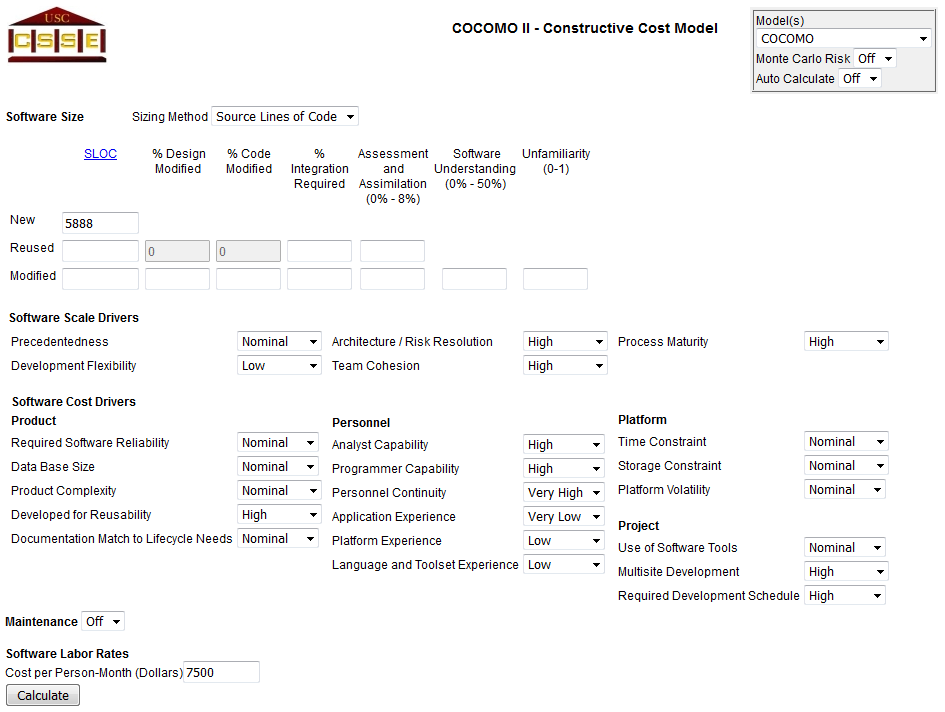
\includegraphics[keepaspectratio=true,scale=0.5]{img/online-cocomo}}
			\vspace{5mm}
		\end{minipage}
	
		\begin{minipage}{\linewidth}
			\vspace{5mm}
			\makebox[\linewidth]{
				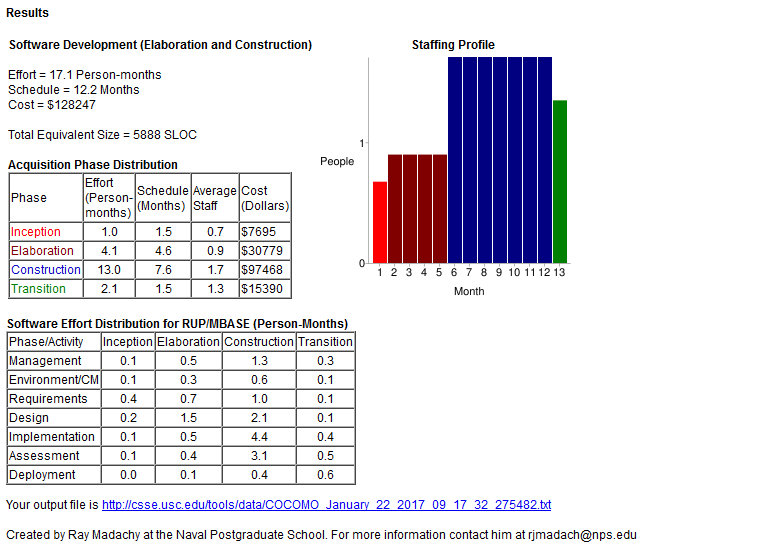
\includegraphics[keepaspectratio=true,scale=0.6]{img/online-cocomo-result}}
			\vspace{5mm}
		\end{minipage}
	
		
		\pagebreak
	\section{Tasks identification}
		The main tasks involving this project are shown in the table below.
		\begin{center}
			\renewcommand{\arraystretch}{1.4}
			\begin{tabular}{ | c | p{4.5cm} | c | c | c |}\hline
			\textbf{Tasks ID} & \textbf{Task} & \parbox[t]{2.2cm}{\textbf{Effort}\\ \bigskip [Person-Days]} & \parbox[t]{2.2cm}{\textbf{Duration}\\ \bigskip [Days]} & \textbf{Dependencies} \\\hline
				T1 & Draft a Project Plan & 20 & 10 & -\\\hline
				T2 & Draft a Requirement Analysis and Specification Document & 40 & 20  & T1\\\hline
				T3 & Draft a Design Document & 40 & 20 & T2\\\hline
				T4 & Develop the software system and write unit tests & 258 & 128 & T3\\\hline
				T5 & Draft a Integration Testing Plan Document & 22 & 12 & T3\\\hline
				T6 & Perform integration testing & 32 & 16 & T4, T5\\\hline
				T7 & Software deployment & 8 & 4 & T6\\\hline
			\end{tabular}
		\end{center}
		\bigskip
		The effort person-days can be calculated using a factor that represent the number of working day in a month that is 19. For \pej the amount of person-days is 420.\\
		Same Tasks shown before are now presented in a Directed Acyclic Graph that help to highlight dependencies among them.
	
		\begin{minipage}{\linewidth}
			\vspace{5mm}
			\makebox[\linewidth]{
				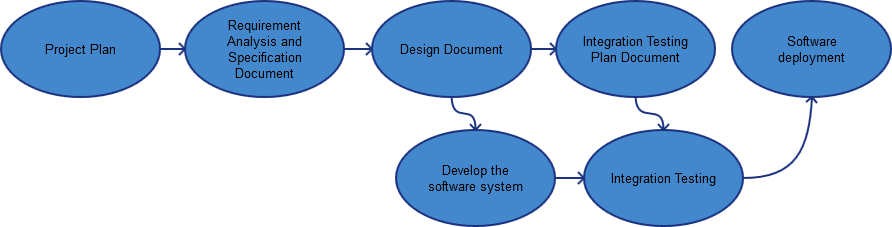
\includegraphics[keepaspectratio=true,scale=0.5]{img/dag}}
			\vspace{5mm}
		\end{minipage}
		\textbf{Observation}: The task T1, contrary to as shown in the table above and in the dag, was started and completed after RASD, DD and ITPD Documents contrary to what normally happens in a real project.
	
		\pagebreak
		
	\section{Task scheduling}
		
		\subsection{Start and Deadlines}
		\subsubsection{Main Tasks}
		\begin{table}[h!]
			\centering
			\begin{tabular}{| c | l | l | l |}
				\hline
				\textbf{Task ID}   &\textbf{Activity}   & \textbf{Start Date}   & \textbf{Deadline} \\
				\hline
				T2 & RASD                & 2016-10-16            & 2016-11-13        \\\hline
				T3 & DD                  & 2016-11-28            & 2016-12-11        \\\hline
				T5 & ITPD                & 2017-01-02            & 2017-01-15        \\\hline
				T1 & PP                  & 2017-01-17            & 2017-01-22        \\\hline
				T4 & Implementation      & 2017-01-23            & 2017-07-31        \\\hline
				T6 & Integration Testing & 2017-08-01            & 2017-08-16        \\\hline
				T7 & Deployment          & 2017-08-17            & 2017-08-22        \\\hline
			\end{tabular}
		\end{table}
		\subsubsection{Implementation Milestone Details}
		\begin{table}[h!]
			\centering
			\begin{tabular}{| c | l | l | l |}
				\hline
				\textbf{Task ID}   &\textbf{Activity}   & \textbf{Start Date}   & \textbf{Deadline} \\
				\hline
				T4.1 &  User Manager development            & 2017-01-23            & 2017-02-10        \\\hline
				T4.2 &  Reservation Manager development     & 2017-02-11            & 2017-03-20        \\\hline
				T4.3 &  Car Manager development             & 2017-03-21            & 2017-04-13        \\\hline
				T4.4 &  Notification development            & 2017-04-14            & 2017-05-09        \\\hline
				T4.5 &  Mobile Interface development        & 2017-05-10            & 2017-06-05        \\\hline
				T4.6 &  Payment Manager development         & 2017-06-06            & 2017-06-29        \\\hline
				T4.7 &  Web Interface development           & 2017-06-30            & 2017-07-31        \\\hline
			\end{tabular}
		\end{table}
		\pagebreak
	
		\subsection{Gantt diagrams}
		Below is shown the Gantt diagram representing the guideline for the scheduling of the project which helps respecting the deadlines and deliverables.\\
		\begin{minipage}{\linewidth}
			\vspace{5mm}
			\makebox[\linewidth]{
				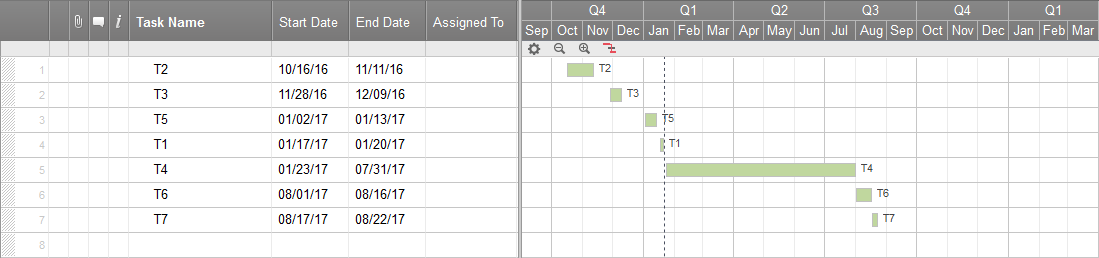
\includegraphics[keepaspectratio=true,scale=0.5]{img/gantt-chart}}
			\vspace{5mm}
		\end{minipage}
		
		Below is shown in details the Gantt diagram of the Implementation Task.\\
		\begin{minipage}{\linewidth}
			\vspace{5mm}
			\makebox[\linewidth]{
				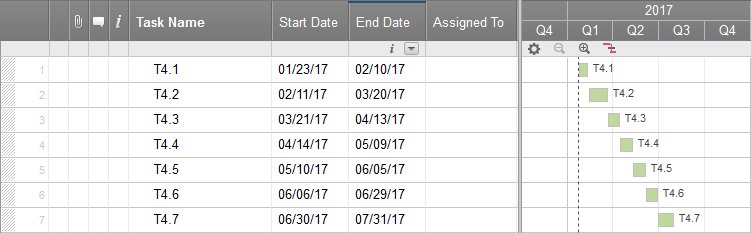
\includegraphics[keepaspectratio=true,scale=0.7]{img/gantt-chart-develop}}
			\vspace{5mm}
		\end{minipage}
		
	\section{Resources allocation}
	As shown in Section 3, thanks to cocomo model, the project will be managed by a team of 2 people. The two developers will work in parallel on each task. This decision is motivated by the risk of lack of staff availability. \\
	During the the software development part the team could be organized in such a way that permit one person to develop the software component while the other one could program the component's unit tests for a better result. In this way in fact the person that create the test does not know how the component is programmed.
	\pagebreak
		
	\section{Risks associated with the project}
		\subsection{Risks}
		The main risk factors related to the project with a probability-of-occurrence are:
		\begin{enumerate}
			\item Delays and Unrealistic schedule
			\item Wrong functionalities
			\item Availability of staff
			\item Bad external components
			\item Integration testing failure
		\end{enumerate}
		\subsection{Solutions}
		\begin{enumerate}
			\item \textbf{Delays and Unrealistic schedule}: the project could require more time than expected. To avoid the problem, the work plan is oversized compared to the estimation with more time for every deadline. If it is not enough it can be release a first, incomplete but working version of the project and build the less essential features later (e.g. starting from the mobile version and develop the web part later).
			\item \textbf{Wrong functionalities}: to avoid misunderstanding about project's functionalities is important to organize, as soon as the project is assigned to the team, many interviews with stakeholders and managers of the project. These interviews should be organized not only during the design part, but also in the development phase too. In this way there is a constant check on the objectives and functionalities, and in case there is the possibility to timely intervention.
			\item \textbf{Availability of staff}: the project could require more time than expected due to illness of key staff at critical times. To avoid the problem, the work plan is oversized compared to the estimation with more time for every deadline, and the highest priority tasks and complex ones are assigned to at least two persons.
			\item \textbf{Bad external components}: the wrong choice about external components (for \pej project are SMS, payment and email services) could cause dependencies with low quality services which could be unreliable or shut-down in the near future. To avoid this, first it is important to choose high quality ones offered by well known companies that have been in the business for years. Second it is important to choose easily replaceable external components.
			\item \textbf{Integration testing failure}: after the implementation of some components, they may not pass the integration testing phase. To mitigate the problem of rewrite the software, it is necessary to define precisely the interfaces between components and subsystems, and by doing integration tests early using stubs and drivers.
		\end{enumerate}
	\pagebreak
	
	\section{Effort Spent}
		\subsection{Hours of work} The time spent to redact this document:
		\begin{itemize}
			\item Bresich Matteo: 30 hours.
		\end{itemize}
		
		\begin{center}
			\begin{tabular}{ | l | l |}
				\hline
				Days & Hours of work\\ \hline
				17/01/17 & 4h\\\hline
				18/01/17 & 4h\\\hline
				19/01/17 & 4h\\\hline
				20/01/17 & 4h\\\hline
				21/01/17 & 6h\\\hline
				22/01/17 & 8h\\\hline
			\end{tabular}
		\end{center}
	\section{References}
		\begin{itemize}
			\item TeXstudio v2.11.2 (http://www.texstudio.org/) to produce this document.
			\item Evolus Pencil v2.0.5 (http://pencil.evolus.vn/) to generate diagrams.
		\end{itemize}
\end{document}